\chapter{Introduction}

\section{Contexte}
La précision du positionnement intérieur reste quelque chose de très important car il peut être utile dans plusieurs domaines comme : La gestion de stocks, la localisation de personnes âgées dans des homes, la localisation chez eux des personnes possédant un bracelet de "prisonnier", etc...

Les systèmes de localisation basés sur GPS souffrent de la détérioration de la précision et sont presque indisponibles dans les environnements intérieurs. Pour les environnements intérieurs, de nombreuses technologies de systèmes de positionnement ont été conçues sur la base de la vision, de la détection infrarouge ou ultrasonore, des champs magnétiques de la terre, des accéléromètres / gyromètres, des balises BLE ou de la communication WiFi. Bien que la création de ces nouvelles applications ait été couronnée de succès, le coût de ces récepteurs, leur consommation d’énergie et leur limitation aux environnements extérieurs excluent de nombreuses applications.

La figure \ref{fig:MethodePos} montre un graphique comparatif de la précision de positionnement concernant différentes technologie \cite{INPOS}. 

\begin{figure}[H]
	\begin{center}
		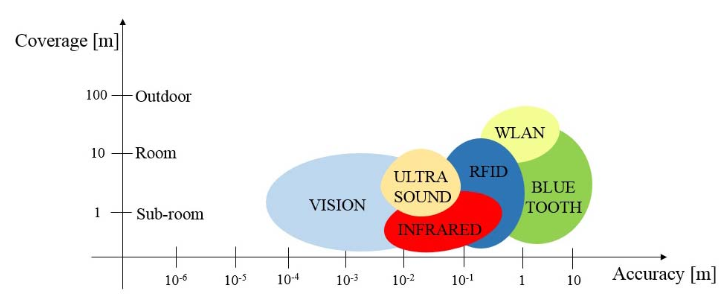
\includegraphics[scale=0.7]{figures/MethodePos.png}
		\caption{Etat de l'art des différentes méthode de positionnement intérieur \cite{INPOS}}
		\label{fig:MethodePos} %% NOTE: always label *after* caption!
	\end{center}
\end{figure}

La géolocalisation avec LoRa est une possibilité séduisante et probablement l'un des meilleurs candidats pour le positionnement intérieur. Le faible coût des infrastructures et des noeuds finaux ainsi que la disponibilité à l'échelle de la ville ou du pays pourraient permettre de nombreuses nouvelles applications. Il n’est donc pas surprenant que les chercheurs et les entités commerciales se soient mis au travail sur ce problème au cours des derniers mois. Cependant, plusieurs défis restent à relever pour qu'un tel système devienne pratique.
Premièrement, la précision de localisation en extérieur qui peut actuellement être atteinte avec LoRa est comprise entre 30 et 50 mètres, ce qui n’est pas suffisant pour de nombreuses applications en milieu urbain. Deuxièmement, très peu d’expérience est disponible pour la conception de systèmes de positionnement intérieurs avec LoRa.

L’objectif général de ce projet est de développer les technologies permettant d'améliorer la précision de la géolocalisation en intérieur sur la base de la technologie LoRa. 

Le positionnement intérieur reste quelque chose de très intéressant et important car il peut être utile dans plusieurs domaines comme : La gestion de stocks, la localisation de personnes âgées dans des homes, la localisation chez eux des personnes possédant un bracelet de "prisonnier", etc...

\section{Aspect Novateur}
Ce travail d'approfondissement doit évaluer une nouvelle approche pour améliorer le positionnement intérieur. En s'appuyant sur les capacités étendues des nouveaux circuits intégrés LoRa, ce projet développera et déploiera un système de localisation capable d'améliorer la précision de la position atteinte par les systèmes de localisation basés sur LoRa existants reposant sur des mécanismes TDOA ou de "ranging". À cette fin, une exploration et une comparaison des différentes techniques "machine learning/deep learning" pour le positionnement basé sur le "fingerprinting" seront effectuées.

L'aspect novateur du projet et d'intégrer un mécanisme d'apprentissage de la position afin d'améliorer la précision. 


\section{Objectifs et tâches à réaliser}
\begin{enumerate}
	\item Etudier le cahier des charges
	\item Etudier l’état de l’art des techniques à utiliser dans le cadre du projet, en particulier les systèmes de localisation indoor basés sur des techniques d’apprentissage, et réunir une documentation (env. 20% effort)
	\item Etablir un planning pour l’ensemble du projet.
	\item Définir un plan des tests à effectuer.
	\item Définir les procédures de test
	\item Définir le setup pour la collecte de données de localisation
	\item Prise en main de l’environnement de développement pour les phases de training et du test de la technique d’apprentissage retenue (e.g., PyTorch).
	\item Implémentation de la solution ML retenue.
	\item Tester le système selon le protocole préétabli.
	\item Faire des propositions pour améliorer les performances de l’algorithme et, si possible, les implémenter.
	\item Rédiger le rapport et documenter l’ensemble du projet.
\end{enumerate}

\section{Structure du rapport}
\todo{Compléter cette partie en fin de rapport quand la structure est définie}



%\begin{enumerate}
%	\item fgfd
%	\item gdgfd
%\end{enumerate}


%\begin{figure}[H]
%	\begin{center}
%		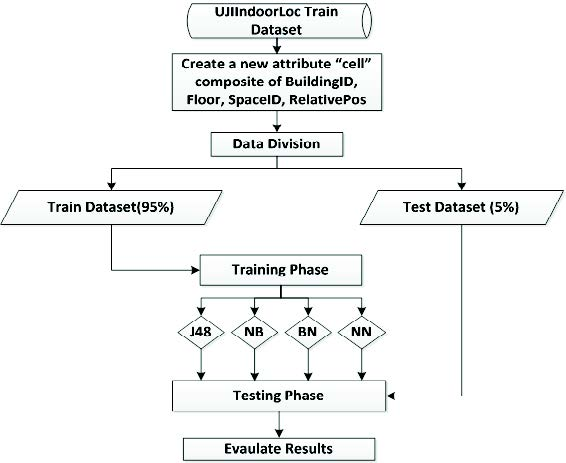
\includegraphics[scale=1]{figures/newattribute.jpg}
%		\caption{The new attribute “cell” construction phase}
%		\label{fig:newAttribute} %% NOTE: always label *after* caption!
%	\end{center}
%\end{figure}

